% Appendix C
 
\chapter{Additional Plots}
\label{appendiximages}
\label{appendix-more-details-on-template}

This appendix provides additional charts that can be helpfull fore more in depth understanding

\section{Dataset Analysis}\label{AppendixDatasetAnalysis}

\begin{figure*}[htb]
    \centering
    \begin{minipage}{1.5\textwidth}
        \centering
        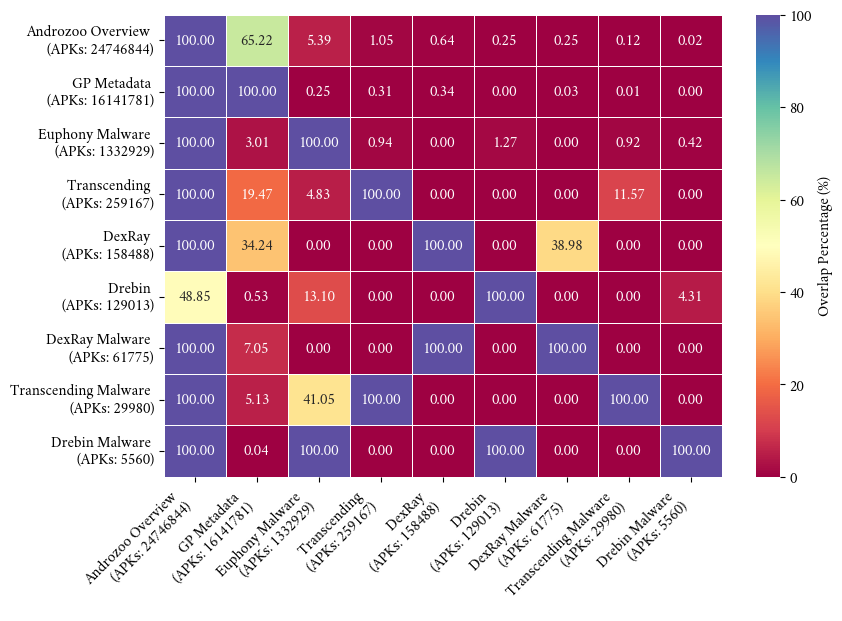
\includegraphics[width=\textwidth]{A_Images/heatmap_sha256_overlaps_percentage.png}
        \captionsetup{width=\textwidth}
        \caption{\label{fig:dataset_overlap}
        Overlap percentages among various Android malware datasets and Google Play metadata provided by \cite{gp_metadata}. 
        The diagonal values represent 100\% overlap (self-comparison), 
        while off-diagonal values highlight shared entries between datasets.
        Notable is that DexRay-, Transcending-, and Drebin Malware are subsets of Androzoo,
        but only partially of Androzoo malware.
        }
    \end{minipage}
\end{figure*}

\newpage

\begin{figure*}[h]
    \centering
    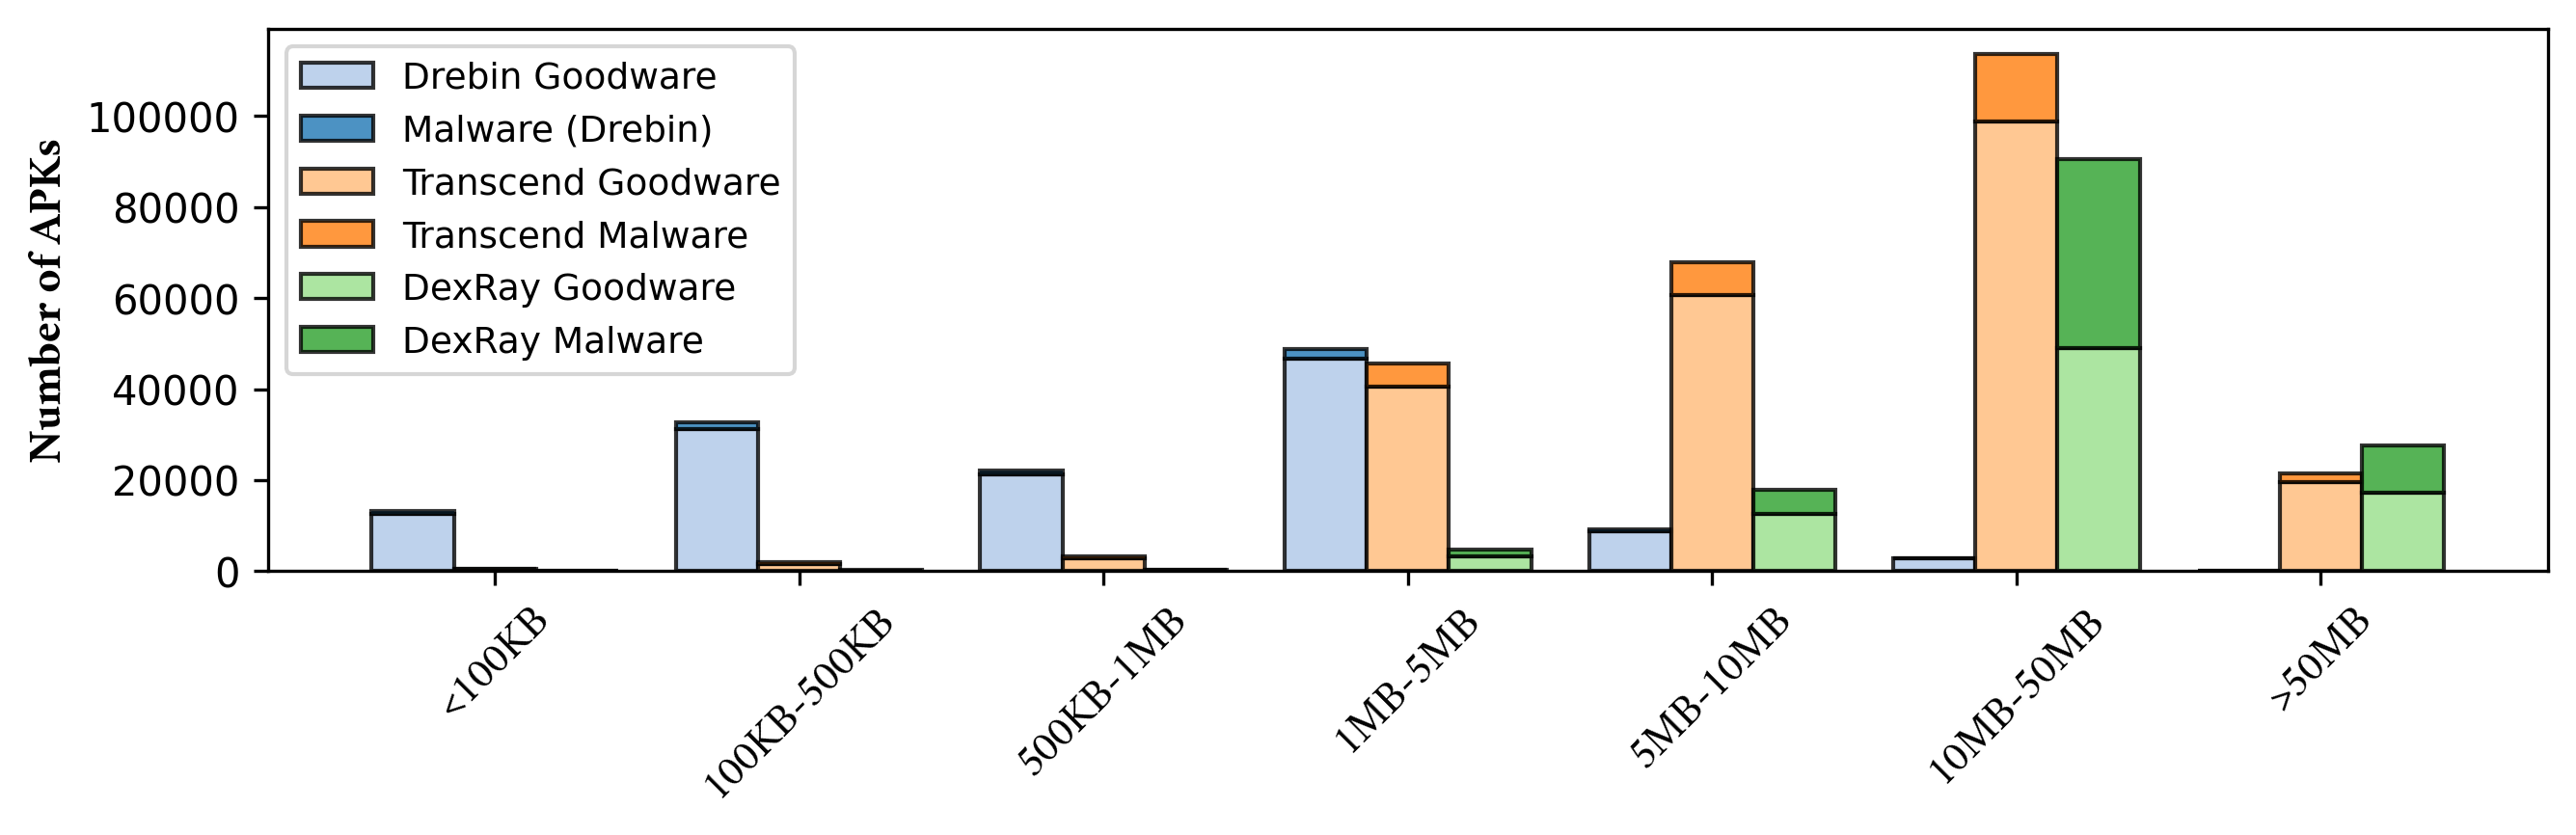
\includegraphics[width=\widefigurewidth]{3_Methodology/dataset_size_distribution.png}
    \caption{\label{fig:dataset_size_evaluation}
    Temporal distribution of Android APKs across three datasets (Drebin, Transcend, and DexRay), 
    categorized into goodware and malware.}
\end{figure*}



\begin{figure*}[b!]
    \centering
    \begin{minipage}{1.5\textwidth}
        \centering
        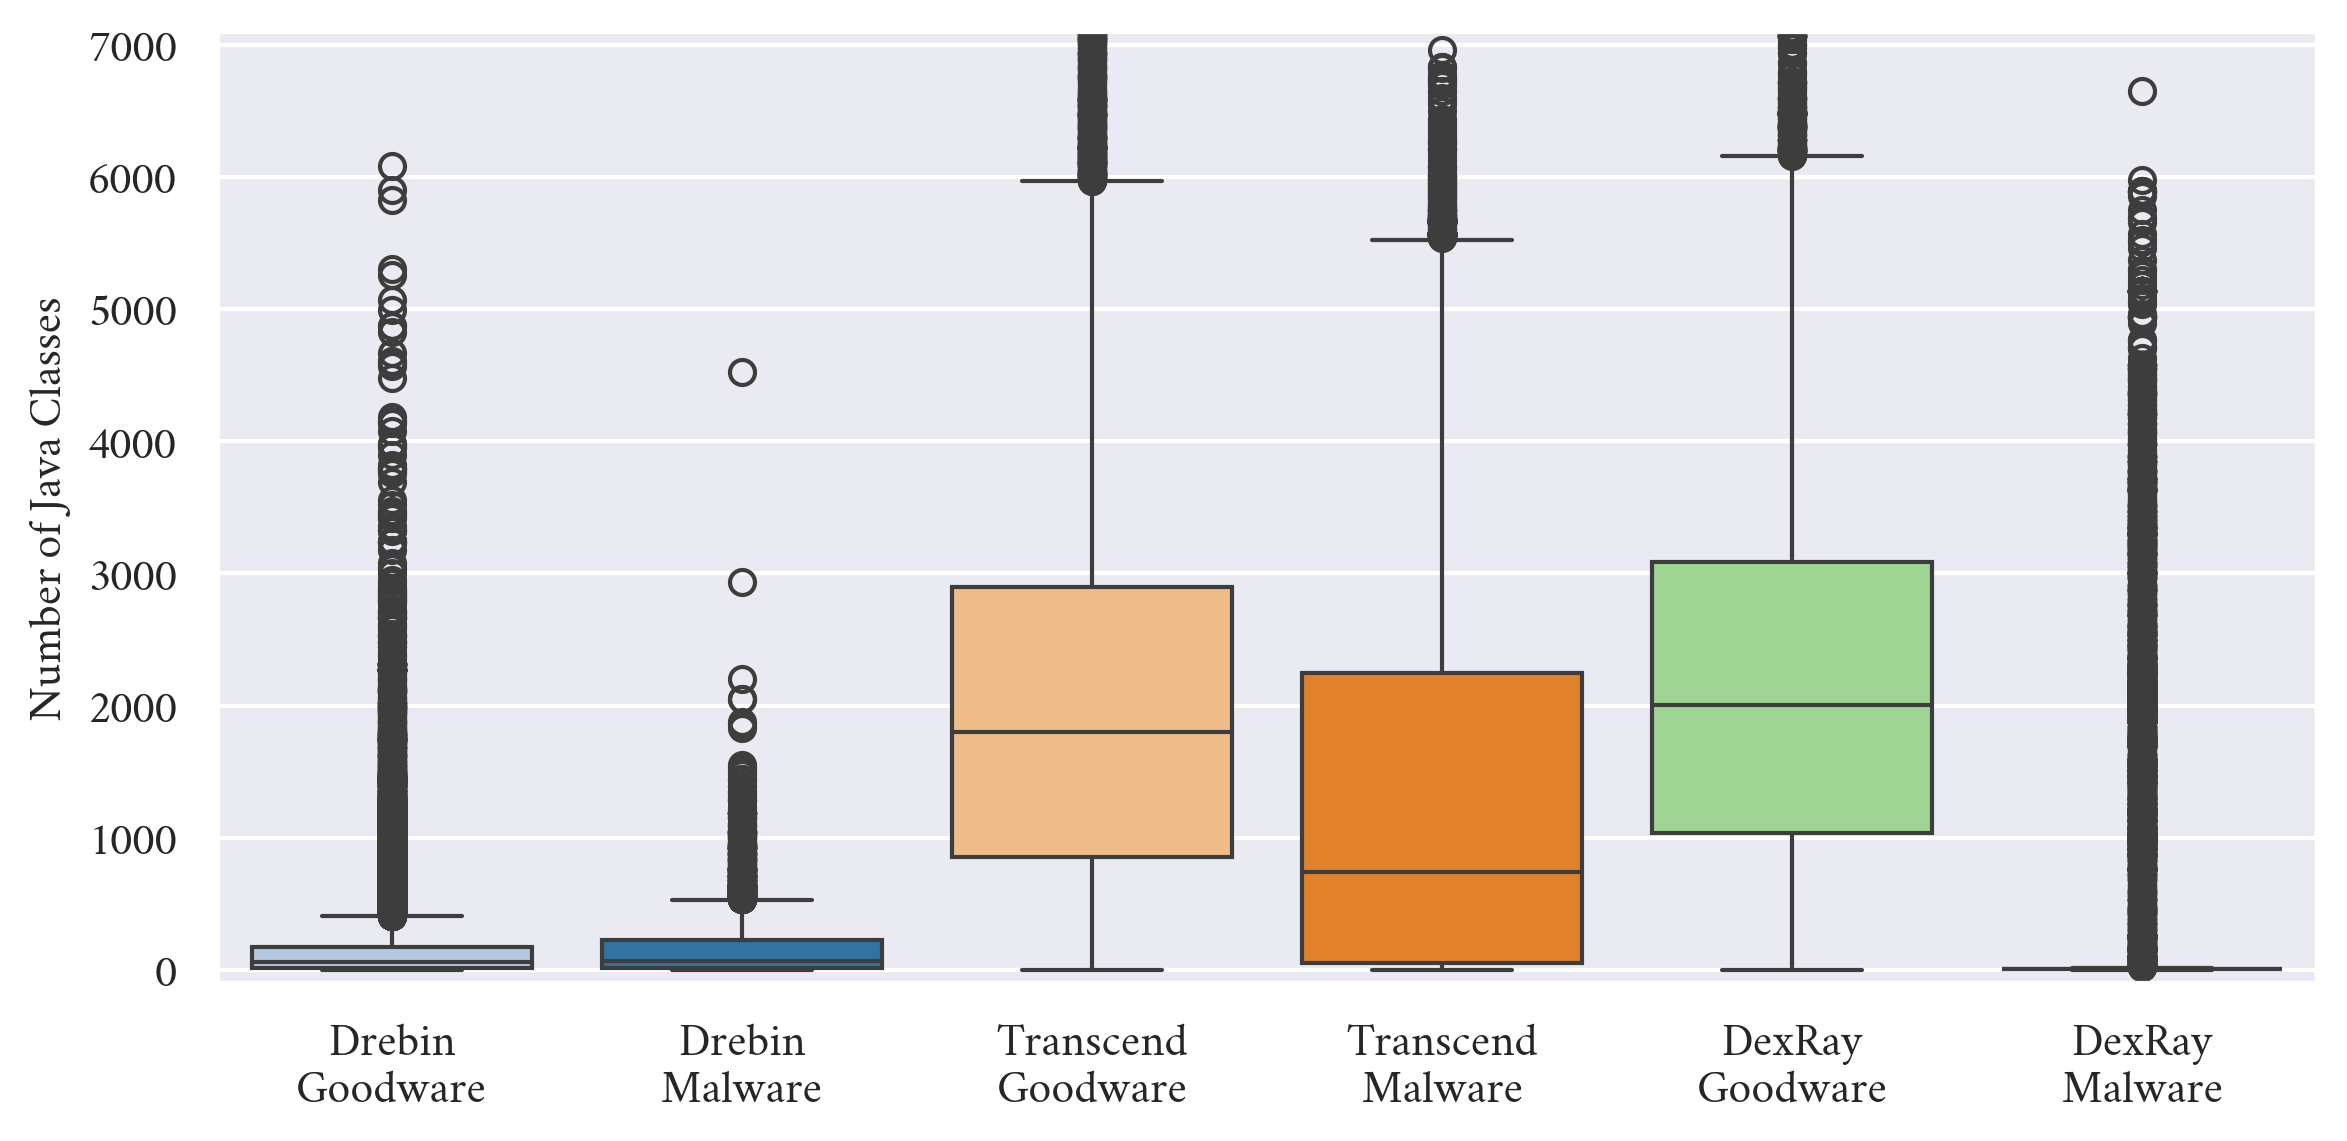
\includegraphics[width=\textwidth]{3_Methodology/java_class_boxplots.png}
        \captionsetup{width=\textwidth}
        \caption{\label{fig:java_class_boxplots}
        The boxplot shows the distribution of Java classes in Android apps 
        across the Drebin, Transcend, and DexRay datasets, 
        split into Goodware and Malware. 
        Drebin and Transcend have an similar java class distribution 
        between Goodware and Malware.
        The DexRay Dataset shows a high inbalance in the number of java classes 
        between the two labels.
        }
    \end{minipage}
\end{figure*}



\begin{table}[]
    \caption{\label{tab:decisiontree}%
    Decision Tree (max\_depth=15) results by dataset and split. Features include Java Classes, Smali Classes, and APK Size.}
    \resizebox{\textwidth}{!}{%
    \begin{tabular}{@{}llcccc@{}}
    \toprule
    \textbf{Dataset} & \textbf{Split} & \textbf{Accuracy} & \textbf{Precision} & \textbf{Recall} & \textbf{F1 Score} \\ \cmidrule(r){1-2} \cmidrule(lr){3-6}
    Drebin         & random     & 90.98\% & 28.13\% & 74.56\% & 40.84\% \\
                   & time based & 80.94\% & 8.99\%  & 37.50\% & 14.50\% \\ \addlinespace
    Transcending   & random     & 88.34\% & 49.57\% & 70.86\% & 58.33\% \\
                   & time based & 85.36\% & 40.46\% & 56.30\% & 47.09\% \\ \addlinespace
    DexRay         & random     & 96.20\% & 96.56\% & 93.74\% & 95.13\% \\
                   & time based & 92.82\% & 85.35\% & 98.30\% & 91.37\% \\
    \bottomrule
    \end{tabular}%
    }
    \end{table}
    
\begin{table}[]
    \caption{\label{tab:decisiontreecombined}%
    Decision Tree (max\_depth=15) results by dataset and split. Features include Java Classes, Smali Classes, APK Size, and Permissions.}
    \resizebox{\textwidth}{!}{%
    \begin{tabular}{@{}llcccc@{}}
    \toprule
    \textbf{Dataset} & \textbf{Split} & \textbf{Accuracy} & \textbf{Precision} & \textbf{Recall} & \textbf{F1 Score} \\ \cmidrule(r){1-2} \cmidrule(lr){3-6}
    Drebin         & random     & 97.10\% & 60.59\% & 89.35\% & 72.21\% \\
                    & time based & 90.66\% & 30.55\% & 91.55\% & 45.81\% \\ \addlinespace
    Transcending   & random     & 92.55\% & 62.81\% & 87.03\% & 72.96\% \\
                    & time based & 91.15\% & 59.08\% & 76.14\% & 66.53\% \\ \addlinespace
    DexRay         & random     & 96.87\% & 96.82\% & 95.21\% & 96.01\% \\
                    & time based & 96.10\% & 91.74\% & 98.82\% & 95.15\% \\
    \bottomrule
    \end{tabular}%
    }
\end{table}

\chapter{Archive}

\begin{table}
    \caption{Java Statistics Summary for DexRay, Transcend, and Drebin}
    \label{tab:statistics}
    \centering
    \footnotesize
    \begin{tabular}{l c c c c c}
        \toprule
        \tabhead{Label} & \tabhead{Q1} & \tabhead{Q3} & \tabhead{Median} & \tabhead{Mean} & \tabhead{Number of Outliers} \\
        \midrule
        \multicolumn{6}{l}{\textbf{Drebin}} \\
        Goodware & 19 & 176 & 60 & 161.83 & 13243 \\
        Malware & 18 & 224 & 66 & 176.87 & 506 \\
        \midrule
        \multicolumn{6}{l}{\textbf{Transcending}} \\
        Goodware & 854 & 2899 & 1800 & 1941.68 & 847 \\
        Malware & 52 & 2244 & 738 & 1312.26 & 996 \\
        \midrule
        \multicolumn{6}{l}{\textbf{DexRay}} \\
        Goodware & 1035 & 3084 & 2007 & 2132.37 & 277 \\
        Malware & 7 & 11 & 11 & 239.98 & 14308 \\
        \bottomrule
    \end{tabular}
\end{table}

\begin{table}
    \caption{Smali Statistics Summary for DexRay, Transcend, and Drebin}
    \label{tab:statistics}
    \centering
    \footnotesize
    \begin{tabular}{l c c c c c}
        \toprule
        \tabhead{Label} & \tabhead{Q1} & \tabhead{Q3} & \tabhead{Median} & \tabhead{Mean} & \tabhead{Number of Outliers} \\
        \midrule
        \multicolumn{6}{l}{\textbf{DexRay}} \\
        Goodware & 16106 & 41352 & 29546 & 28603.12 & 0 \\
        Malware & 445 & 817 & 598 & 4113.59 & 13704 \\
        \midrule
        \multicolumn{6}{l}{\textbf{Transcend}} \\
        Goodware & 13145 & 40372 & 25364 & 27234.10 & 1 \\
        Malware & 764 & 25015 & 7057 & 15912.92 & 605 \\
        \midrule
        \multicolumn{6}{l}{\textbf{Drebin}} \\
        Goodware & 331 & 2353 & 901 & 2275.87 & 14288 \\
        Malware & 173 & 2316 & 805 & 2161.74 & 899 \\
        \bottomrule
    \end{tabular}
\end{table}
